\section{用户地址空间}
\begin{figure}[htb]
    \centering
    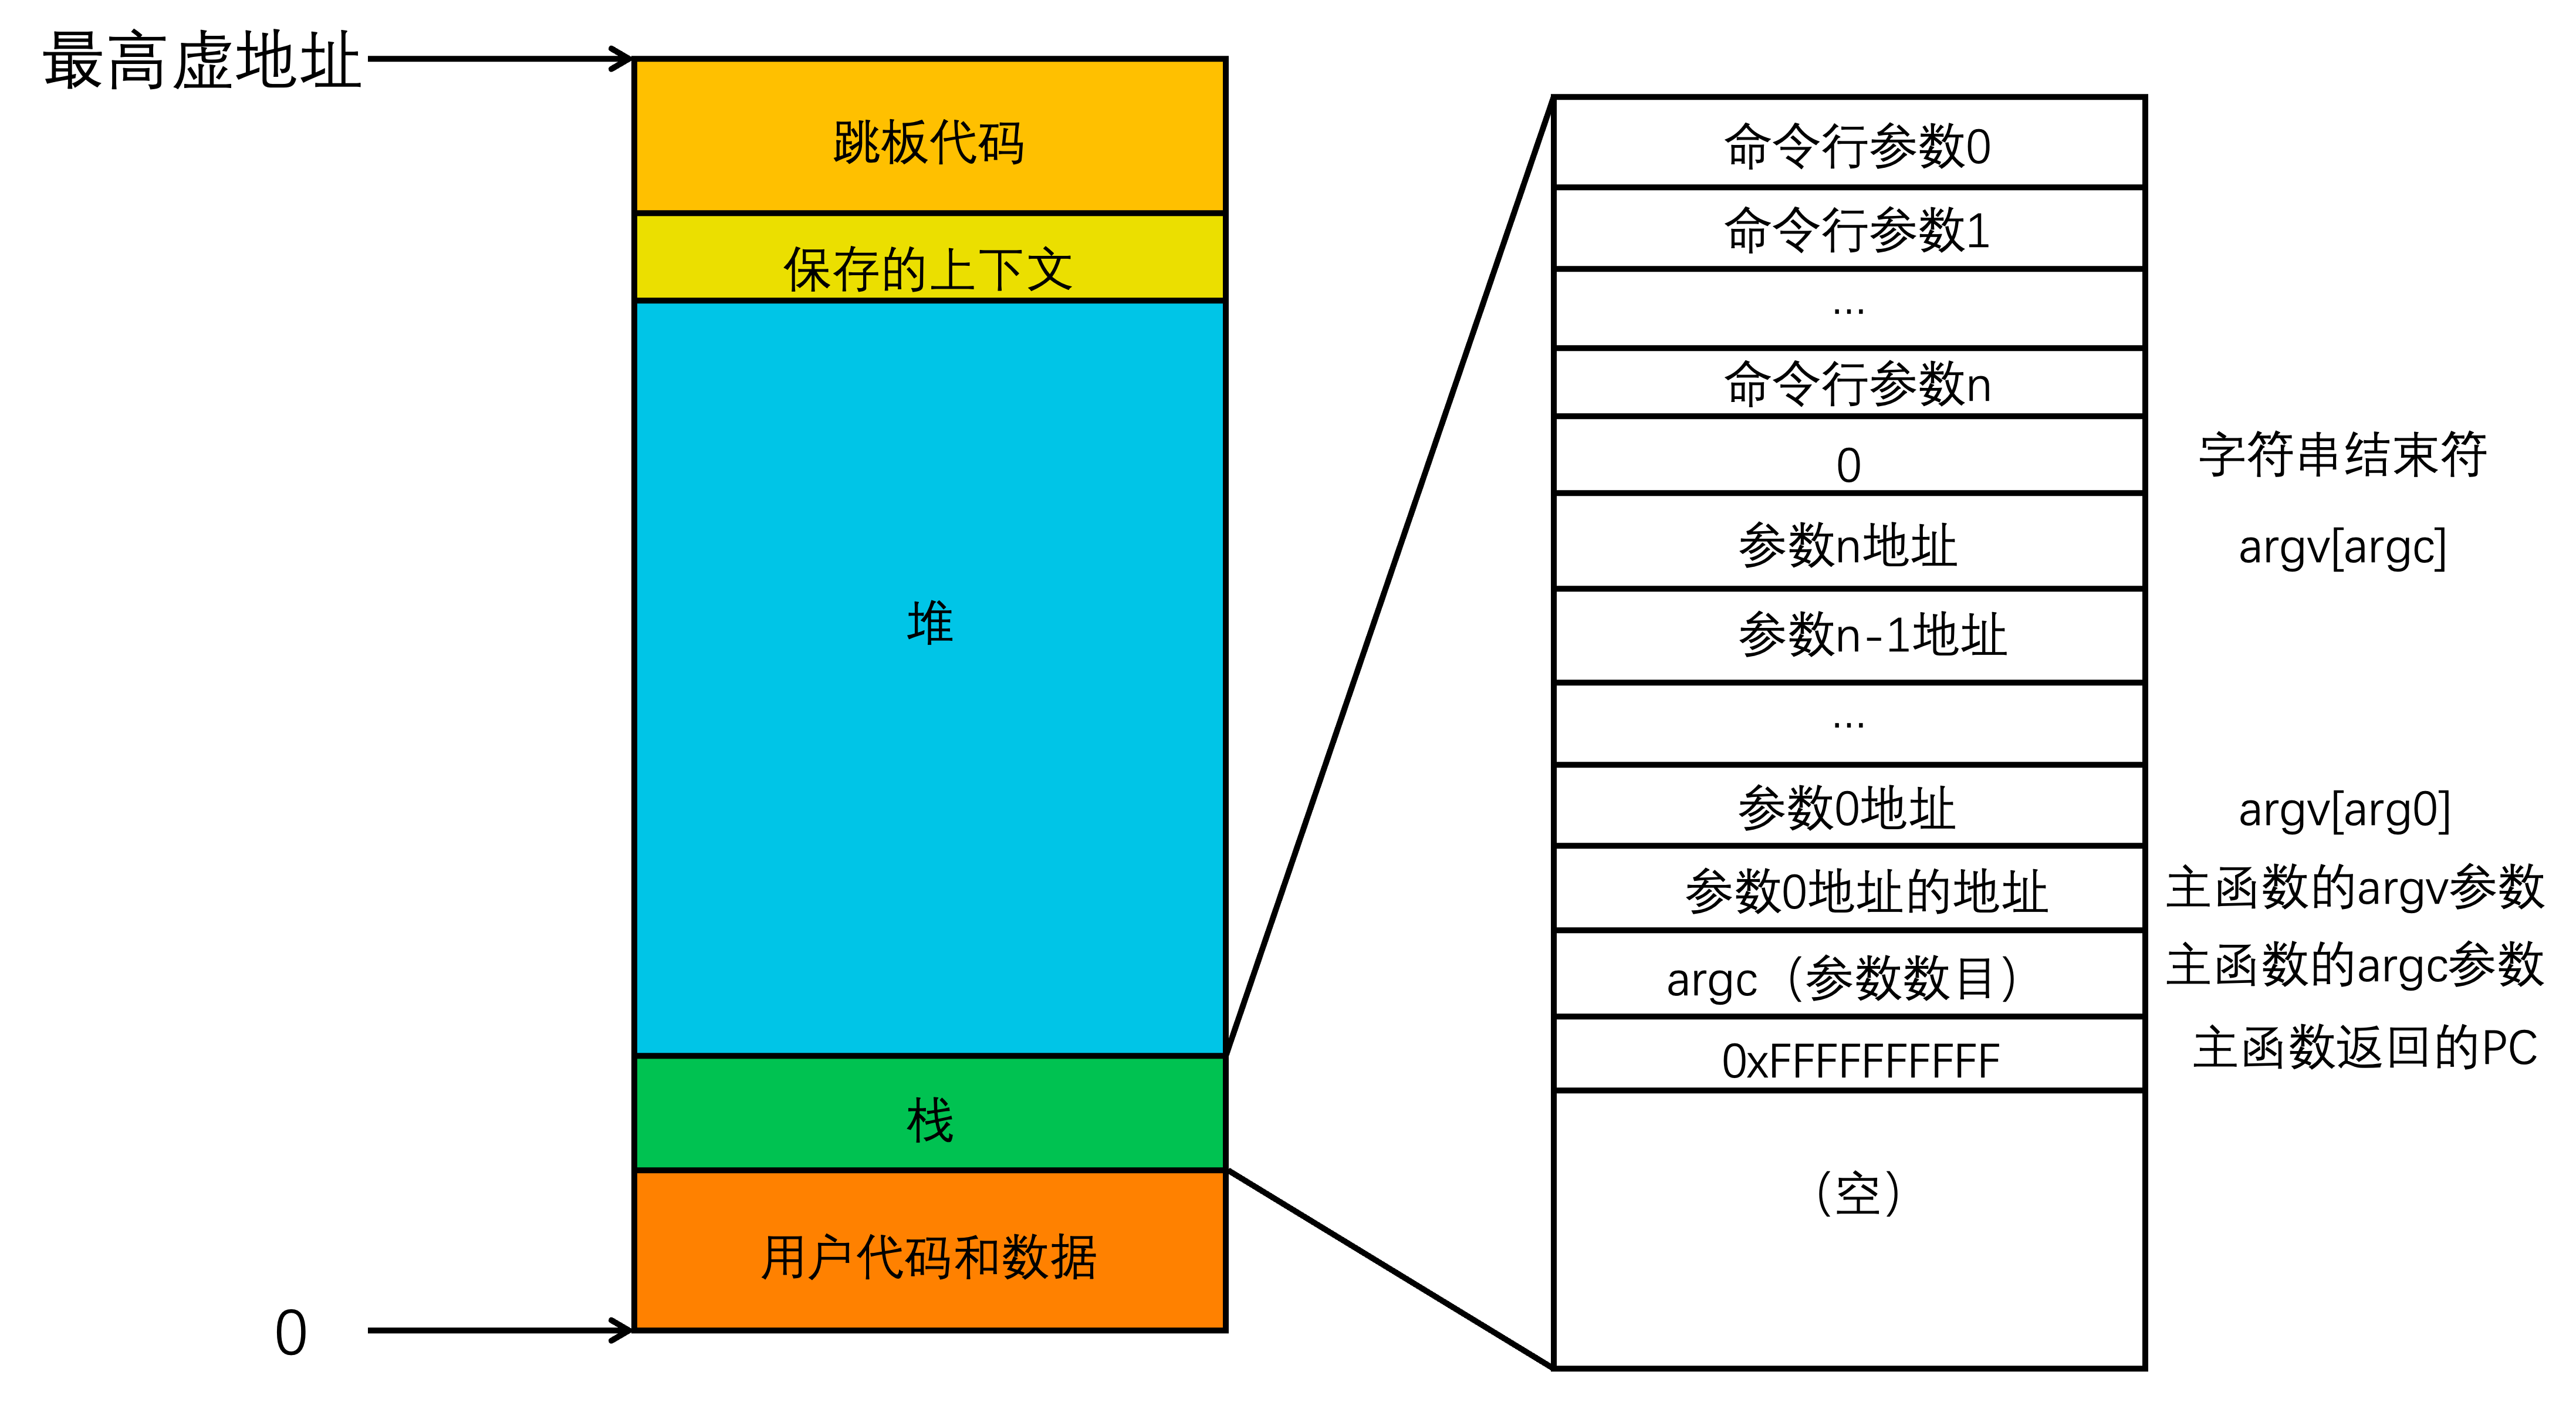
\includegraphics[width=\textwidth]{figures/04-04-用户地址空间示意图.png}
    \caption{
        用户虚拟地址空间示意
    }
    \label{fig:user virtual process}
\end{figure}
每一个进程都有一个独立的页表,当npucore实现进程切换的时候,对应的页表也会切换。

当一个用户进程通过系统调用向操作系统请求更多的用户空间时,npucore首先在os/src/frame_allocator.rs中的StackFrameAllocator的基于栈的数据结构实现空闲物理页的分配,然后将物理页的映射加入到用户的页表当中。
npucore将设置PTEflags::R,PTEflags::W,PTEflags::U,PTEflags::X以及PTEflags::V标志位到对应的页表项目,使得用户可以对分配的页面进行读写操作。
大多数的用户进程并不能完全利用所有的虚拟空间,对于没有用到的空间,它对应的页表项PTEflags::V标志位始终为0。

页表的设计有很多的好处。首先,首先不同的进程使用不同的页表,相同的虚拟地址映射到不同的物理地址,因此每一个进程可以拥有自己独立的内存空间。其次,用户的虚拟地址是连续的,对应的物理地址不一定是连续的,这样可以有效的避免内存碎片。最后,内核将所有的用户的跳板代码都映射到了同一段虚地址,可以有效的实现上下文切换。

如图\ref{fig:user virtual process}所示,用户的虚拟地址空间被分为了三个部分,分别是用户代码段,用户数据段以及用户堆栈段。用户代码段用于存放用户的代码,用户数据段用于存放用户的数据,用户堆栈段用于存放用户的堆栈。
其中,用户栈的初始内容如图中所示,由execve函数完成初始化,其中包含了用户的命令行参数和返回地址,紧接着就是main函数使用的栈空间。
堆是动态内存分配的区域,用于存储在运行时分配的数据。在npucore中,堆的起始地址通常在数据段结束后,并根据需要进行扩展。通过系统调用(如mmap和sbrk),用户程序可以动态地管理堆内存。
栈是用于存储函数调用和局部变量的区域。在npucore中,栈从高地址向低地址生长,通常位于用户地址空间的顶部。栈的大小可以通过操作系统配置或在运行时动态调整。。

代码段是存储进程执行指令的区域。在npucore中,代码段通常从虚拟地址0开始,并包含可执行程序的指令。这个区域对应于用户程序的文本部分。
数据段包含了全局变量和静态变量等数据。npucore将数据段安排在代码段之后,从一个虚拟地址开始,并在运行时动态地分配和使用。

用户在代码段执行用户程序,将elf指定的数据段内容存放在相应的数据段位置。因为我们对与内核的映射是直接映射,所以操作系统对于用户的地址空间是直接可见的。
同时,堆栈段的大小是动态变化的,当用户程序需要更多的堆栈空间时,会通过系统调用向操作系统请求更多的堆栈空间,操作系统会在用户的地址空间中分配更多的堆栈空间,并将堆栈空间映射到用户的地址空间中

npucore实现了execve来将elf文件加载到内存的进程地址空间中,实现了sbrk来动态的分配用户空间,实现了mmap来将文件映射到用户空间,实现了munmap来取消文件的映射。
execve将elf文件中程序所规定的代码和数据加载到内存中,然后操作系统需要建议对应的映射,从而实现了用户地址空间的建立。


\subsection{sbrk系统调用}
sbrk系统调用是早期的Unix系统中的一个系统调用,用于动态的分配用户空间。sbrk系统调用的原型如下:
\begin{lstlisting}[language=c]
    void *sbrk(intptr_t increment);
\end{lstlisting}
sbrk系统调用将堆的大小增加increment字节,并返回堆的起始地址。
如果increment为负数,则堆的大小减少increment字节。如果堆的大小超过了进程的地址空间,则sbrk系统调用返回-1,并设置errno为ENOMEM。
sbrk系统调用可以为一个进程扩大或者缩小堆的大小,主要的实现是由os/src/memory_set.rs中的sbrk函数完成。
sbrk函数调用Memoryset::mmap或者Memoryset::munmap来实现堆的扩大或者缩小。
mmap函数不仅用于sbrk系统调用,还用于mmap系统调用,用于将文件映射到用户空间和开辟匿名内存映射。
\begin{lstlisting}[language=rust,caption={sbrk}]
    pub fn sbrk(&mut self, heap_pt: usize, heap_bottom: usize, increment: isize) -> usize {
        let old_pt: usize = heap_pt;
        let new_pt: usize = old_pt + increment as usize;
        // 判断扩大堆还是缩小堆
        if increment > 0 {
            let limit = heap_bottom + USER_HEAP_SIZE;
            if new_pt > limit {
                return old_pt;
            } else {
                self.mmap(
                    old_pt,
                    increment as usize,
                    MapPermission::R | MapPermission::W | MapPermission::U,
                    MapFlags::MAP_ANONYMOUS | MapFlags::MAP_FIXED | MapFlags::MAP_PRIVATE,
                    1usize.wrapping_neg(),
                    0,
                );
                trace!("[sbrk] heap area expanded to {:X}", new_pt);
            }
        } else if increment < 0 {
            // 如果缩小后的堆地址小于堆底地址,则不进行缩小
            if new_pt <= heap_bottom {
                return old_pt;
            } else {
                self.munmap(old_pt, increment as usize).unwrap();
            }
        }
        new_pt
    }
\end{lstlisting}
sbrk的实现依赖于函数mmap的实现,将在接下来的章节介绍,mmap是比sbrk更加灵活的系统调用,能狗处理更复杂的内存分配和使用的情况。


\subsection{mmap}
\begin{lstlisting}[language=rust,caption={sys_mmap}]
    pub fn sys_mmap(
        start: usize,
        len: usize,
        prot: usize,
        flags: usize,
        fd: usize,
        offset: usize,
    ) -> isize
\end{lstlisting}
参数start:指向欲映射的内存起始地址,通常设为 NULL,代表让系统自动选定地址,映射成功后返回
该地址。
\begin{itemize}
    \item 参数len:代表将文件中多大的部分映射到内存。
    \item 参数prot:映射区域的保护方式。
    \item 参数flags:影响映射区域的各种特性。在调用mmap()时必须要指定MAP_SHARED 或MAP_PRIVATE。MAP_FIXED 如果参数start所指的地址无法成功建立映射时,则放弃映射,不对地址做修正。通常不鼓励用此旗标。
    MAP_SHARED对映射区域的写入数据会复制回文件内,而且允许其他映射该文件的进程共享。MAP_PRIVATE 对映射区域的写入操作会产生一个映射文件的复制,即私人的“写入时复制”(copy on
    write)对此区域作的任何修改都不会写回原来的文件内容。MAP_ANONYMOUS建立匿名映射。此时会忽略参数fd,不涉及文件,而且映射区域无法和其他进程共
    享。MAP_DENYWRITE只允许对映射区域的写入操作,其他对文件直接写入的操作将会被拒绝。MAP_LOCKED 将映射区域锁定住,这表示该区域不会被置换(swap)。
    \item 参数fd:要映射到内存中的文件描述符。如果使用匿名内存映射时,即flags中设置了MAP_ANONYMOUS,fd设为-1。
    \item 参数offset:文件映射的偏移量,通常设置为0,代表从文件最前方开始对应,offset必须是分页大小的整数倍。
    \item 返回值:若映射成功则返回映射区的内存起始地址,否则返回-1。
\end{itemize}

\begin{figure}[htb]
    \centering
    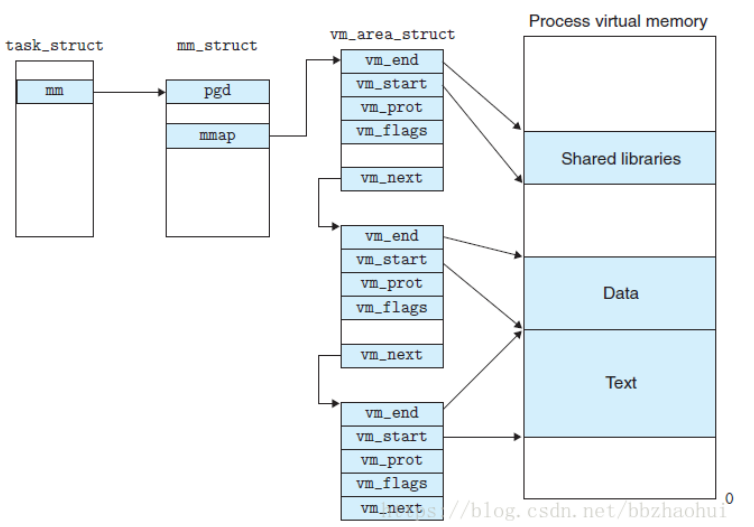
\includegraphics[width=\textwidth]{figures/04-04-内存地址空间.png}
    \caption{
        内存地址空间
    }
    \label{fig:内存地址空间}
\end{figure}

mmap用于把文件映射到用户空间中,简单说mmap就是把一个文件的内容在内存里面做一个映像。映
射成功后,用户对这段内存区域的修改可以直接反映到内核空间,同样,内核空间对这段区域的修改也
直接反映用户空间。那么对于内核空间<---->用户空间两者之间需要大量数据传输等操作的话效率是非
常高的。进程可以像读写内存一样对普通文件的操作。mmap系统调用使得进程之间通过映射同一个普
通文件实现共享内存。
UNIX网络编程第二卷进程间通信对mmap函数进行了说明。该函数主要用途有三个:
1、将一个普通文件映射到内存中,通常在需要对文件进行频繁读写时使用,这样用内存读写取代I/O读
写,以获得较高的性能;
2、将特殊文件进行匿名内存映射,可以为关联进程提供共享内存空间;
3、为无关联的进程提供共享内存空间,一般也是将一个普通文件映射到内存中。
第一步:找到最后一次mmap映射区域
\begin{lstlisting}[language=rust]
    let idx = self.last_mmap_area_idx();
\end{lstlisting}
每个进程所申请的用户地址空间是用vector存储的vm_area_struct的结构体,其中start和end就是代表
这一个area虚拟地址的开始和结束,而我们的结构体在vector中是按照虚拟地址升序排序的,也就是说
我们会找到最后一个符合要求的vector下标


第二步:mmap获取映射区域的起始地址,如果设置了MAP_FIXED,则会直接使用用户的参数start,
不对地址做修正。
\begin{lstlisting}[language=rust,caption={mmap}]
    let start_va: VirtAddr = if flags.contains(MapFlags::MAP_FIXED) {
        // unmap if exists
        self.munmap(start, len);
        start.into()
    }
\end{lstlisting}
如果没有设置,mmap就会拿到先前得到的最后一次mmap映射区域。如果设置了MAP_PRIVATE 或者
MAP_ANONYMOUS,就直接将要新映射的区域new_area与最后一次mmap映射区域合并并返回,没
有设置就会将最后一次mmap映射区域的末尾作为新映射的区域的起始。而新映射的区域的末尾则根据
用户参数len设置。
\begin{lstlisting}[language=rust,caption={mmap}]
    else {
        if let Some(idx) = idx {
        let area = &mut self.areas[idx];
        if flags.contains(MapFlags::MAP_PRIVATE | MapFlags::MAP_ANONYMOUS)
        && prot == area.map_perm
        && area.map_file.is_none()
        {
        let end_va: VirtAddr = area.inner.vpn_range.get_end().into();
        area.expand_to(VirtAddr::from(end_va.0 + len)).unwrap();
        return end_va.0 as isize;
        }
        area.inner.vpn_range.get_end().into()
        } else {
        MMAP_BASE.into()
        }
        };
        let mut new_area = MapArea::new(
        start_va,
        VirtAddr::from(start_va.0 + len),
        MapType::Framed,
        prot,
        None,
    );
        
\end{lstlisting}
第三步:mmap会判断是否是文件映射,即是否包含MAP_ANONYMOUS。如果没有包含,就会先获取
fd_table,并根据用户参数fd从fd_table找到对应的文件描述符,这里文件相关内容不作赘述。然后设
置文件偏移量offset并置入new_area中
\begin{lstlisting}[language=rust,caption={mmap}]
    if !flags.contains(MapFlags::MAP_ANONYMOUS) {
        let fd_table = task.files.lock();
        match fd_table.get_ref(fd) {
        Ok(file_descriptor) => {
        if !file_descriptor.readable() {
        return EACCES;
        }
        let file = file_descriptor.file.deep_clone();
        file.lseek(offset as isize, SeekWhence::SEEK_SET).unwrap();
        new_area.map_file = Some(file);
        }
        Err(errno) => return errno,
        }
    }
\end{lstlisting}
第四步:mmap将new_area加入到先前的vector中,而且需要保持原vector的有序性,这里使用了rust
语言的特性。
\begin{lstlisting}[language=rust,caption={mmap}]
    let (idx, _) = self
    .areas
    .iter()
    .enumerate()
    .skip_while(|(_, area)| {
    area.inner.vpn_range.get_start() >= VirtAddr::from(MMAP_END).into()
    })
    .find(|(_, area)| area.inner.vpn_range.get_start() >= start_va.into())
    .unwrap();
    self.areas.insert(idx, new_area);
\end{lstlisting}

\subsection{execve}
应用程序自身的角度来看,进程 (Process) 的一个经典定义是一个正在运行的程序实例。当程序运行在操作系统中的时候,从程序的视角来看,它会产生一种“幻觉”:即该程序是整个计算机系统中当前运行的唯一的程序,能够独占使用处理器、内存和外设,而且程序中的代码和数据是系统内存中唯一的对象。体表现为“进程”这个抽象概念。站在计算机系统和操作系统的角度来看,并不存在这种“幻觉”。事实上,在一段时间之内,往往会有多个程序同时或交替在操作系统上运行,因此程序并不能独占整个计算机系统。具体而言,进程是应用程序的一次执行过程。并且在这个执行过程中,由“操作系统”执行环境来管理程序执行过程中的 **进程上下文** – 一种控制流上下文。这里的进程上下文是指程序在运行中的各种物理/虚拟资源(寄存器、可访问的内存区域、打开的文件、信号等)的内容,特别是与程序执行相关的具体内容:内存中的代码和数据,栈、堆、当前执行的指令位置(程序计数器的内容)、当前执行时刻的各个通用寄存器中的值等。
\begin{figure}[htb]
    \centering
    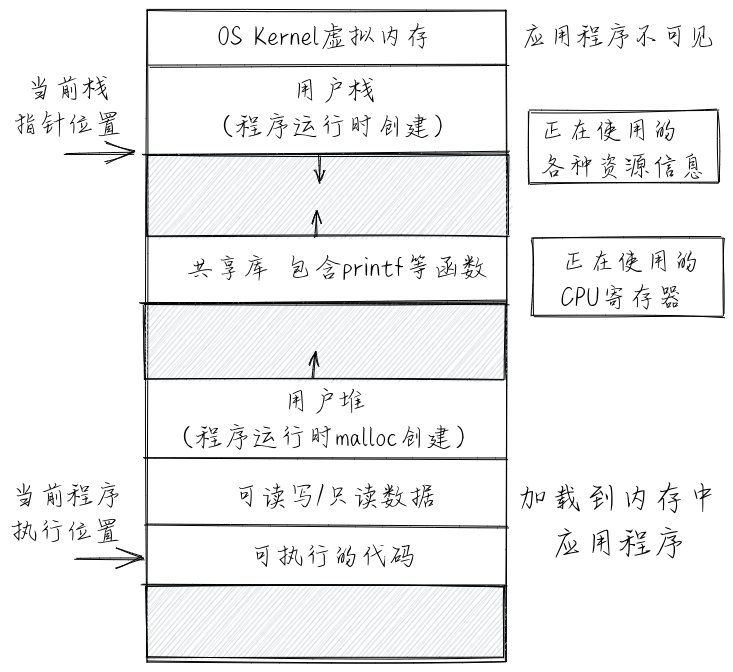
\includegraphics[width=\textwidth]{figures/04-04-进程的地址空间.png}
    \caption{
        进程的地址空间
    }
    \label{fig:进程的地址空间}
\end{figure}

exec 用一个新的程序来代替当前进程的内存和寄存器,但是其文件描述符、进程 id 和父进程都是不变的。
它根据文件系统中保存的某个文件来初始化用户部分。`exec`通过 `open()`打开二进制文件。然后,它读取 ELF 头。应用程序以通行的 ELF 格式来描述。一个 ELF 二进制文件包括了一个 ELF 头,然后是连续几个程序段的头。
exec 会检查文件是否包含 ELF 二进制代码。一个 ELF 二进制文件是以4个“魔法数字”开头的,即 0x7F,“E”,“L”,“F”。如果 ELF 头中包含正确的魔法数字,`exec` 就会认为该二进制文件的结构是正确的。

\begin{lstlisting}[language=rust,caption={execve}]
    pub fn sys_execve(
        pathname: *const u8,
        mut argv: *const *const u8,
        mut envp: *const *const u8,
    ) -> isize
\end{lstlisting}
execve()的前置条件
fork()复制某一个进程,为execve()的执行,准备条件。
execve()的核心工作:
参数转换,将argv,envp转为Vec<String>。
open()打开path路径下的可执行文件,对其进行检查。
load_elf()将其加载到当前的空间中。
load_elf的核心工作:
将elf文件映射到内核空间的`MMAP_BASE`地址处。
在map_elf()中,把elf文件的内容拷贝到用户的MemorySet中
